
%%%%%%%%%%%%%%%%%%%%%%% file typeinst.tex %%%%%%%%%%%%%%%%%%%%%%%%%
%
% This is the LaTeX source for the instructions to authors using
% the LaTeX document class 'llncs.cls' for contributions to
% the Lecture Notes in Computer Sciences series.
% http://www.springer.com/lncs       Springer Heidelberg 2006/05/04
%
% It may be used as a template for your own input - copy it
% to a new file with a new name and use it as the basis
% for your article.
%
% NB: the document class 'llncs' has its own and detailed documentation, see
% ftp://ftp.springer.de/data/pubftp/pub/tex/latex/llncs/latex2e/llncsdoc.pdf
%
%%%%%%%%%%%%%%%%%%%%%%%%%%%%%%%%%%%%%%%%%%%%%%%%%%%%%%%%%%%%%%%%%%%


\documentclass[runningheads,a4paper]{llncs}

\usepackage{amssymb}
\setcounter{tocdepth}{3}
\usepackage{graphicx}

\usepackage{url}

\selectlanguage{slovene}

\urldef{\mailsa}\path|{matej.hrlec.fri, gal.kos.fri}@gmail.com|    
\newcommand{\keywords}[1]{\par\addvspace\baselineskip
\noindent\keywordname\enspace\ignorespaces#1}

% CUSTOM IMPORTS
% fixed image postion
\usepackage{float}
\usepackage[export]{adjustbox}

\begin{document}

\mainmatter  % start of an individual contribution

% first the title is needed
\title{Interaktivni projekt s pomočjo uporabo CNN}

% a short form should be given in case it is too long for the running head
\titlerunning{Interaktivni projekt s pomočjo uporabo CNN}

% the name(s) of the author(s) follow(s) next
%
% NB: Chinese authors should write their first names(s) in front of
% their surnames. This ensures that the names appear correctly in
% the running heads and the author index.
%
\author{Matej Hrlec, Gal Kos}
%
% (feature abused for this document to repeat the title also on left hand pages)

% the affiliations are given next; don't give your e-mail address
% unless you accept that it will be published
\institute{Fakulteta za računalništvo in informatiko,\\
Večna pot 113, 1000 Ljubljana\\}

%
% NB: a more complex sample for affiliations and the mapping to the
% corresponding authors can be found in the file "llncs.dem"
% (search for the string "\mainmatter" where a contribution starts).
% "llncs.dem" accompanies the document class "llncs.cls".
%

\toctitle{CNN}
\tocauthor{Authors' Instructions}
\maketitle


\begin{abstract}
Ker obstaja precej knjižnic, ki uporabljajo konvolucijske nevronske mreže za obdelavo podatkov, bomo v okviru tega projekta naredili pregled te panoge strojnega učenja in naredili praktično implementacijo s pomočjo Android aplikacije. Uporabljene bodo funkcionalnost prenosa sloga umetniških slik, ohranjanje barve pri prenosu in klasificiranju objektov v slikah.
%\keywords{We would like to encourage you to list your keywords within
%the abstract section}
\end{abstract}


\section{Uvod}
V zadnjih letih se je začel nagel razvoj sistemov strojnega učenja, ki temeljijo na simuliranju človeškega razmišljanja. To je v veliki možno zaradi velikega napredka na področju programerskih vmesnikih za izvajanje masovno paralelizirane kode na grafičnih karticah. Poleg tega so se kapacitete grafičnih pomnilnikov in pomnilniških povezav precej povečale, kar omogoča obdelavo velikih podatkovnih baz.

V okviru tega projekta se bova osredotočila na uporabo konvolucijskih nevronskih mrež, bolj natančno na njihovo uporabo pri obdelavi in klasifikaciji slik. Z uporabo in povezovanjem knjižnic, ki podpirajo določene operacije nad slikami, želiva narediti mobilno aplikacijo, s pomočjo katere bi lahko uporabnik izkoristil vse te funkcionalnosti.

\raggedbottom
\section{Opis tematike in pregled področja}

\subsection{Nevronske mreže}
Umetne nevronske mreže (angl. \textit{Artificial neural networks} - ANNs) so računski model, ki temelji na veliki zbirki povezav preprostih nevronskih enot oziroma nevronov (angl. \textit{artificial neurons}), ki so po obnašanju sorodni možganskim aksonom\cite{wiki:ANN}. 

Vsaka nevronska enota je povezana z mnogimi drugimi, povezave lahko povečajo ali zavirajo stanje aktiviranja sosednjih nevronskih enot. Posamezna nevronska enota izračunava izhode s pomočjo funkcije seštevanja. Pogosto obstaja tudi pragovna funkcija (angl. threshold function) na vsaki povezavi ali na enoti sami, ki določa stopnjo, ki jo mora signal preseči preden se lahko razširi do sosednjih nevronov. Nevronski sistemi se odločanja naučijo samostojno, tako da niso eksplicitno programirani in se odlikujejo predvsem na področjih, kjer je rešitev ali zaznavanje značilnosti težko izraziti v tradicionalnem računalniškem programu.

Nevronske mreže so običajno sestavljene iz več plasti, pri čemer se signalna pot razteza od prve (vhodne) do zadnje (izhodne) plasti nevronskih enot kot je vidno na sliki \ref{fig:layersANN}. Sodobna nevronska omrežja so v smislu simulacije pretočnejša, zato pri tovrstnih omrežjih povezave interaktirajo veliko bolj kaotično in kompleksno. Najnaprednejše so dinamične nevronske mreže, ki lahko na podlagi pravil tvorijo nove povezave in celo ustvarjajo nove nevronske enote ali jih onemogočajo.

\begin{figure}[H]
\centering
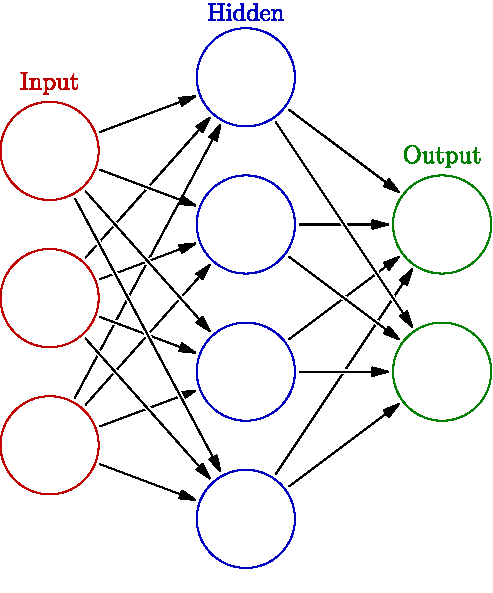
\includegraphics[width=55mm]{figures/Colored_neural_network.pdf}
% ref: https://en.wikipedia.org/wiki/Artificial_neural_network#/media/File:Colored_neural_network.svg
\caption{Vhodna, skrita in izhodna plast pri umetnih nevronskih mrežah}
\label{fig:layersANN}
\end{figure}

Cilj nevronskih mrež je reševanje problemov na enak način, kot bi jih reševali človeški možgani, čeprav so veliko bolj abstraktne. Sodobni projekti, ki uporabljajo nevronske mreže, ki so običajno sestavljene iz nekaj tisoč do nekaj milijonov povezav, kar je še vedno velikokrat manj kompleksno od človeških možganov in so bolj podobne računski moči črva.

Zanimiv vidik nevronskih sistemov je, da so nepredvidljivi glede tega, kako uspešni bodo pri samostojnem učenju. Po tem, ko se naučijo na učnih podatkih, nekateri dobro rešujejo probleme, medtem ko drugi pri reševanju novih problemov niso tako uspešni. Proces učenja običajno zahteva več tisoč ciklov interakcije. Podobno kot pri ostalih metodah strojnega učenja, torej sistemih, ki se učijo iz podatkov, so tudi nevronske mreže uporabljajo za reševanje širokega spektra različnih nalog, kot sta računalniški vid in prepoznavanje govora, ki sta težko rešljiva problema z uporabo navadnega na pravilih temelječega programiranja.

\subsection{Konvolucijske nevronske mreže}

Konvolucijske nevronske mreže (angl. \textit{convolutional neural network} - CNN) so vrsta umetnih nevrosnkih mrež, pri katerih se vzorec povezljivosti med nevronskimi enotami zgleduje po ureditvi vidnega korteksa pri živalih\cite{wiki:CNN}. Posamezni kortikalni nevroni se odzivajo na dražljaje v omejeni prostorski regiji oziroma receptivnem polju. Tovrstna polja različnih nevronov se delno prekrivajo, tako da vidno polje razdelijo na ploščice. Odziv posameznega nevrona na dražljanje v svojem receptivnem polju lahko matematično aproksimiramo z operacijo konvolucije. Konvolucijska omrežja izhajajo iz bioloških procesov in so variacije večplastnih zaznav, ki katerih je predprocesiranje minimalno. Konvolucijske nevronske mreže se uporabljajo v aplikacijah za prepoznavo slik in videa, v priporočilnih sistemih in pri obdelavi naravnega jezika.

Konvolucijske nevronske mreže so torej različice večslojnih zaznavanj (angl. \textit{multilayer perceptron} - MLP), ki so osnovane tako, da lahko posnemajo vidni korteks. Mreže CNN imajo naslednje značilne lastnosti:
\begin{itemize}
\item \textbf{3D volumni nevronov:} Sloji CNN imajo nevrone razporejene v treh dimenzijah: širina, dolžina in globina, kot je vidno na sliki \ref{fig:layersCNN}. Nevroni znotraj sloja so povezani samo z majhnim območjem plasti pred njih - receptivnim poljem. Različni tipi plasti, tako lokalno kot globalno povezani, so nakopičeni, s čimer tvorijo arhitekturo CNN.

\item \textbf{Lokalna povezljivost:} V skladu s konceptom receptivnih polj mreže CNN izkoriščajo prostorsko-lokalno korelacijo z uveljavljanjem lokalne povezljivosti med nevroni sosednjih plasti. Arhitektura tako zagotavlja, da naučeni filtri ustvarijo najmočnejši odziv na prostorsko-lokalni vhodni vzorec. Kopičenje več takih plasti vodi do nelinearnih filtrov, ki postajajo vedno bolj globalni, torej se odzivajo na vedno večje območje. To omogoča omrežju, da najprej ustvari dobre predstavitve manjših delov vhoda in nato te majhne dele združi v predstavitve večjih področij.

\item \textbf{Deljene uteži:} Pri mrežah CNN je vsak filter repliciran v celotnem vidnem polju. Te replicirane enote si delijo enako parametrizacijo, torej vektor uteži in začetno vrednost, s čimer tvorijo mapo značilk. Tako vsi nevroni v dani konvolucijski plasti zaznavajo povsem enako funkcijo. Takšno podvajanje nevronskih enot omogoča, da so lastnosti detektirane ne glede na njihov položav v vidnem polju, kar predstavlja translacijsko invarianco.
\end{itemize}

\begin{figure}[H]
\centering
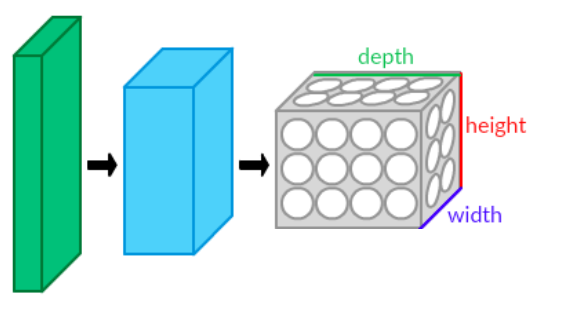
\includegraphics[width=80mm]{figures/Conv_layers.png}
% ref: https://en.wikipedia.org/wiki/Convolutional_neural_network#/media/File:Conv_layers.png
\caption{Plasti CNN so razporejene v treh dimenzijah (širina, dolžina in globina)}
\label{fig:layersCNN}
\end{figure}

Skupaj zgornje lastnosti omogočajo mrežam CNN doseganje boljše generalizacije problemov. Delitev uteži dramatično zmanjša število prosti parametrov, ki se jih je potrebno naučiti, s čimer znižuje pomnilniške zahteve za delovanje mreže. Zmanjšanje zahtev po virih omogoča učenje večjih in močnejših nevronskih omrežij. Na sliki \ref{fig:archCNN} referenco je vidna tipična arhitektura CNN.

\begin{figure}[H]
\centering
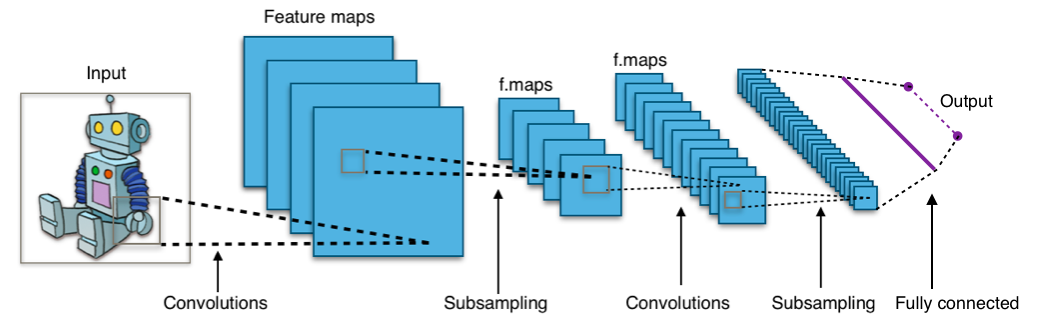
\includegraphics[width=120mm]{figures/Typical_cnn.png}
% ref: https://en.wikipedia.org/wiki/Convolutional_neural_network#/media/File:Typical_cnn.png
\caption{Tipična arhitektura konvolucijskih nevronskih mrež}
\label{fig:archCNN}
\end{figure}

\subsection{Projekt Darknet}
Darknet je odprtokodno ogrodje (angl. \textit{framework}) za delo z nevronskimi mrežami programirano v jeziku C in platformi CUDA (angl. \textit{Compute Unified Device Architecture})\cite{darknet13}. Ogrodje podpira procesorsko in grafično podprto računanje.

Darknet – YOLO (angl. \textit{you only look once}) je realnočasovni sistem za zaznavanje objektov na slikah s pomočjo mrež CNN, ki lahko zazna preko 9000 kategorij objektov. 

Sistem uporablja enotno nevronsko omrežje na celotni sliki, s čimer razdeli sliko na regije, napove omejitvena polja in verjetnosti za vsako regijo. Omejitvena polja so utežena z napovedano verjetnostjo. Sistem detektira celotno sliko v času testiranja, zato so napovedi izračunane glede na globalni kontekst slike. Sistem natisne objekte, ki jih je zaznal in izračuna zaupanje (angl. \textit{confidence}) in kako dolgo je trajalo da je objekta našel. V okviru projekta je na voljo več pred-naučenih modelov.  Primer detekcije je viden na sliki \ref{fig:darknetExample}.

\begin{figure}[H]
\centering
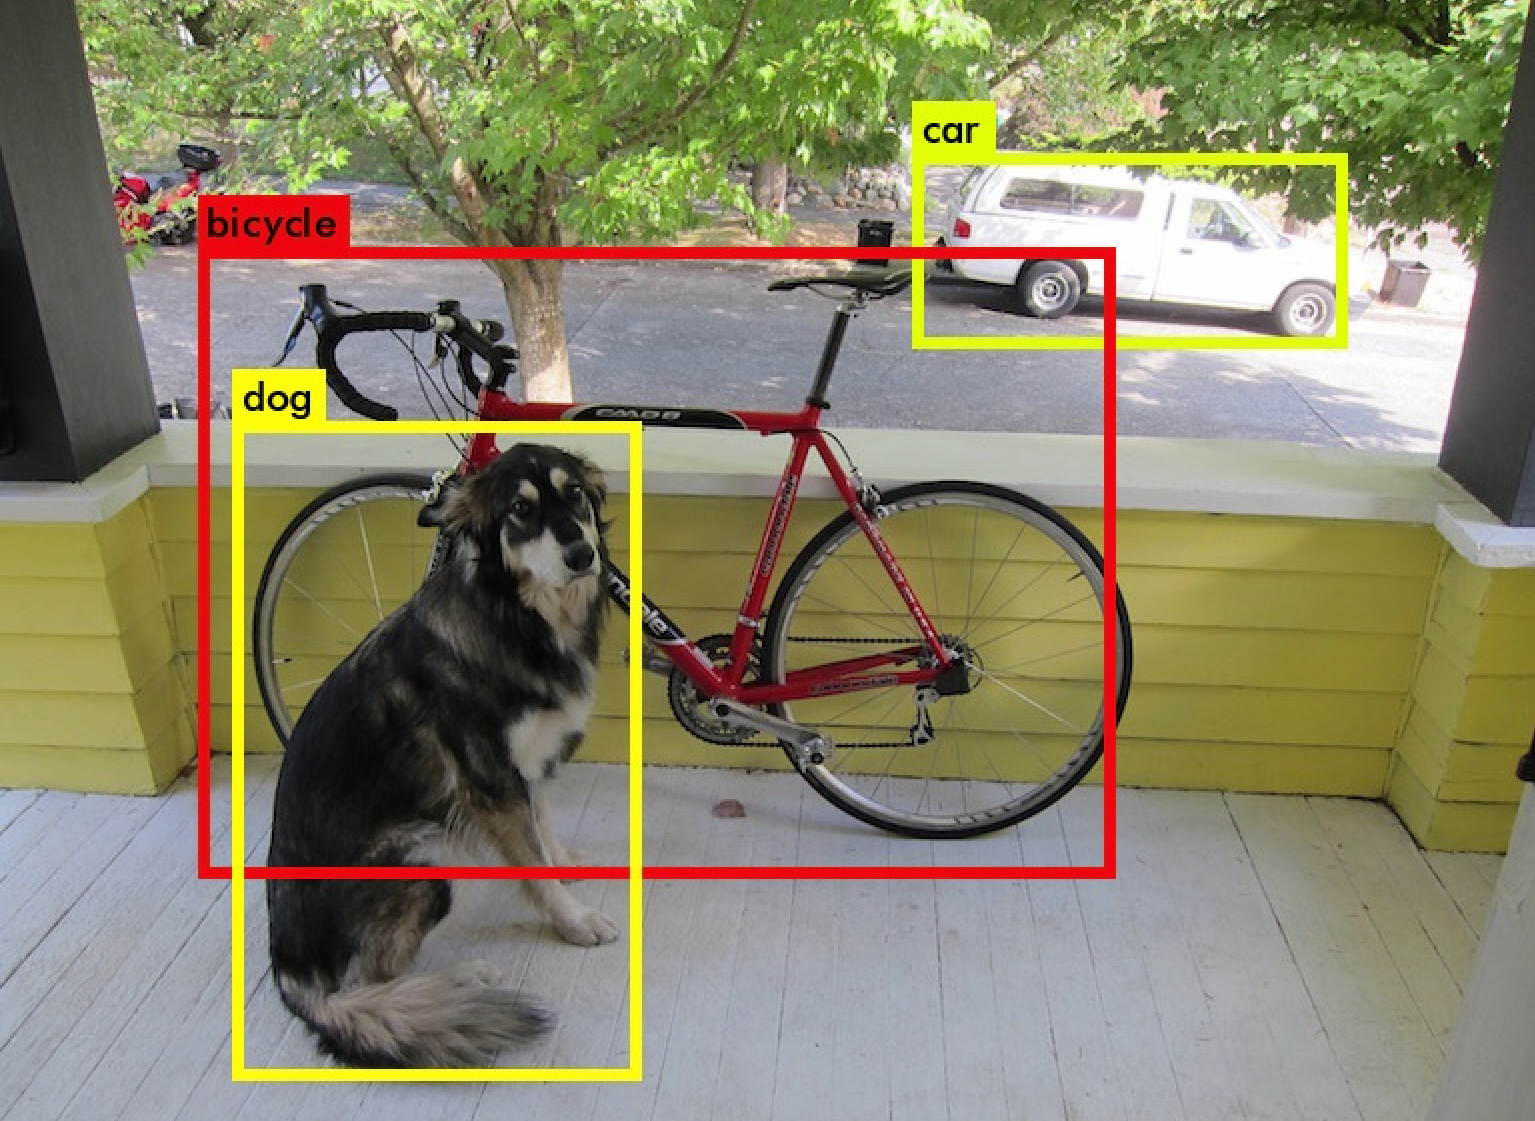
\includegraphics[width=90mm]{figures/darknetExample.png}
% https://pjreddie.com/media/image/Screen_Shot_2016-11-17_at_11.14.54_AM.png
\caption{Primer detekcije z uporabo sistema Darknet - YOLO}
\label{fig:darknetExample}
\end{figure}

\subsection{TenserFlow}
S pomočjo uporabe odprtokodne programske knjižnice lahko razvijamo sisteme, ki so sposobni grajenja in učenja nevronskih mrež. S tem lahko omogočimo zaznavanje vzorcev in povezav, podobno temu, ki smo ga sposobni ljudje.

Arhitektura API-ja omogoča uporabo CPE (centralna procesna enota) ali GPE (grafična procesna enota) na stacionarnih računalnikih, strežnikih in mobilnih napravah. Z njeno uporabo zgeneriramo vozlišča in graf, kjer povezave predstavljajo matematične operacije. Robovi grafov predstavljajo večdimenzionalne nize podatkov, s katerimi komunicirajo. Ta model lahko potem ostale knjižnjice uporabljajo za klasificiranje različnih vhodnih podatkov, kot je prepoznavanje govora, objektov v sliki,…

\subsubsection{CUDA}
Za razvijalce in znanstvenike so postali moderni GPE zelo zanimivi, saj nudijo dovolj funkcionalnosti in moči, da jih lahko uporabljamo računsko intenzivne aplikacije. \textit{Nvidia} je za svoje grafične kartice razvila napreden jezik in orodje \textit{CUDA}, ki temelji na standardu \textit{OpenCV}, ki nudi povezavo med izvajanjem kode na CPE in GPE.

Pomemben del računalniškega vida je obdelava slik, področje, za katerega so bili grafični pospeševalci namenjeni. Druge uporabe tudi temeljijo na masovni paralelizaciji računanja in se jih zato pogosto da prenesti na GPE arhitekture z ohranjanjem konceptualne konsistence glede na funkcionalnost na CPE.

\subsection{Prenos sloga slike z uporabo CNN}
\label{sub:prenos_sloga}

\begin{figure}
\centering
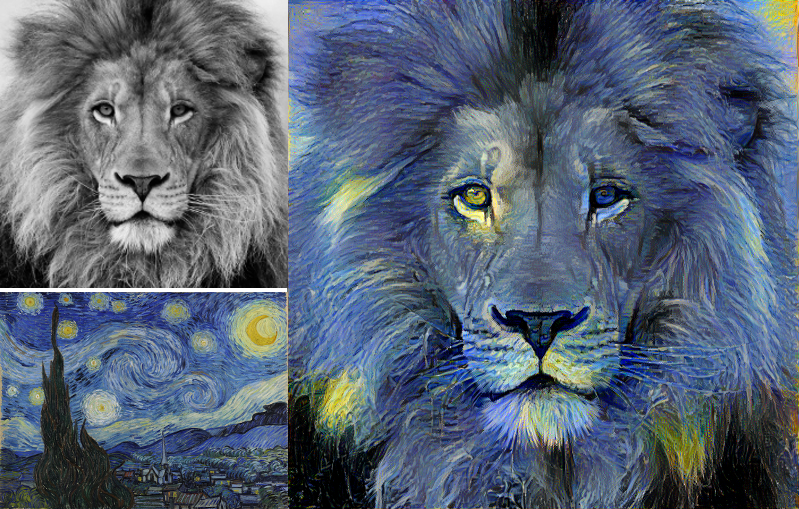
\includegraphics[width=110mm]{figures/prenos_sloga.png}
% ref: https://github.com/cysmith/neural-style-tf
\caption{Primer uporabe prenosa sloga slike z uporabo CNN}
\label{fig:prenos_sloga}
\end{figure}

V zadnjih letih je bilo precej razvoja za prenos sloga z uporabo globokih nevronskim mrež. Gatys et al. \cite{prenos_sloga} so predlagali pristop, ki uporabi inovativen pristop k zaznavi slog umetniške slike in njenega prenosa na druge slike. S pomočjo tega algoritma ohranjajo slog nanosov s čopičem, geometrijskih oblik in slikarskih struktur. Uporabljajo visoko nivojsko predstavitev lastnosti skrite plasti, ki jo dobimo z CNN. Vsebina in slog slike se podata kot dva ločena vhoda v algoritem, zato lažje dobimo model umetniškega sloga. To dosežejo z oblikovanjem optimizacijskega problema, ki se začne reševat z belim platnom. Nato po korakih išče novo podobo, ki bi sprožila podobne nevronske aktivacije kot vsebina slike in podobne korelacije lastnosti, izraženo z Gramovo matriko.

\subsection{Ohranjanje barve slike}

\begin{figure}
\centering
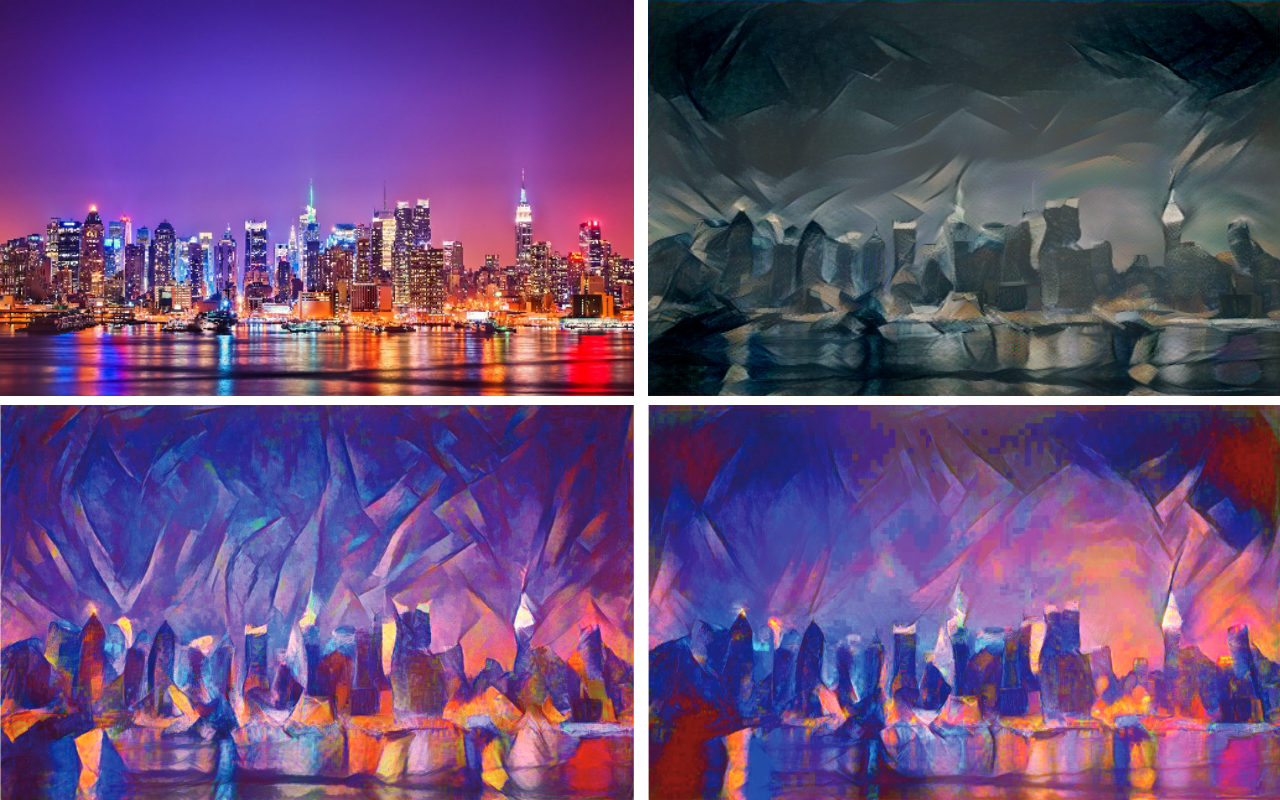
\includegraphics[width=120mm]{figures/prenos_barve.png}
% ref: https://github.com/cysmith/neural-style-tf
\caption{Primer ohranjanje barve pri prenosu sloga slike z uporabo CNN. Na spodnji levi sliki je prikazan postopek z ujemanjem barvnega histograma, na sliki desno spodaj pa prenos sloga z uporabo svetlosti}
\label{fig:prenos_barve}
\end{figure}

Z uporabo prej opisanega postopka \ref{sub:prenos_sloga} dobimo kvalitetno preslikavo slikarskega sloga, vendar hkrati izgubimo tudi barve na originalni sliki. Gatys et al. \cite{prenos_barve} so se lotili tega problema z dvema pristopoma: 

\begin{itemize}
\item \textbf{ujemanje barvnega histograma:} linearen prenos barve izbrane slike na umetniško sliko, preden jo podamo v nevronsko mrežo. Pri tem smo omejeni s kvaliteto prenosa barv, ki je težji pri bolj različnih slikah. Poleg tega se pri združevanju ohranijo vsebinske strukture slike, predvsem ostre poteze na umetniški sliki.

\item \textbf{prenos sloga z uporabo svetlosti:} iz obeh slik se prenese plast svetlosti, nad katerima se potem uporabi algoritem nevronskih mrež. Izhod potem združimo z barvo originalne slike, s čimer dobimo končno sliko. S tem popolno ohranimo barve, vendar se izgubi povezava med plastjo svetlosti in barve pri umetniški slike. To se opazi predvsem pri močnih potezah čopiča, ki jim ta postopek lahko da cel spekter barv. S tem postopkom poleg tega tudi optimiziramo grajenje nevronske mreže, saj zmanjšamo nabor parametrov za eno tretjino.
\end{itemize}

\section{Realizacija projekta}

\subsection{Miselni vzorec ideje izvedbe projekta}

% https://app.mindmup.com/map/_free/eda28ee0130411e7a10a3343dba65313
\begin{figure}[H]
\centering
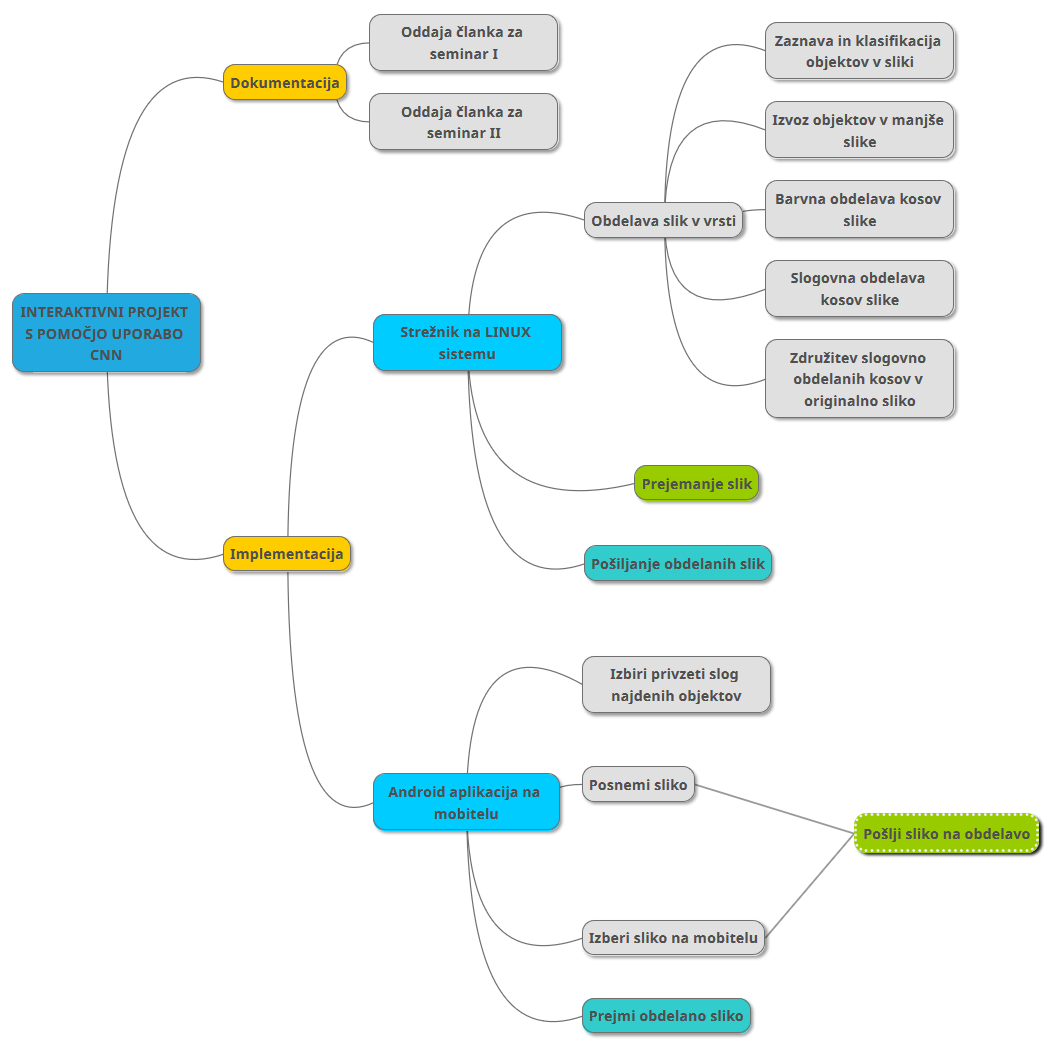
\includegraphics[width=150mm, center]{figures/mind_map.png}
% ref: https://github.com/cysmith/neural-style-tf
\caption{Miselni vzorec ideje izvedbe projekta}
\label{fig:mind_map}
\end{figure}

\subsection{Opis projektne zasnove}
V sklopu tega projekta bomo razvili sistem, ki bo s pomočjo knjižnic, ki uporabljajo mreže CNN, obdeloval fotografije. 
Na čelnem delu (angl. \textit{frontend}) bomo razvili \textit{Android} aplikacijo, ki bo omogočala zajem fotografije s pomočjo kamere ali izbor slike na pomnilniku telefona. Ko bo uporabnik fotografijo zajel, jo bo aplikacija poslala na strežnik, kjer bo fotografija nadalje obdelana s pomočjo različnih zgoraj omenjenih knjižnic glede na zahteve uporabnikove. V zaledju (angl. \textit{backend}) bomo implementirali strežnik, ki bo stregel zahtevke \textit{Android} uporabnikov in koordiniral uporabo knjižnic CNN. Ko bo fotografija na strežniku dokončno obdelana, jo bo strežnik skupaj z ostalimi detekcijskimi podatki modificirano vrnil uporabniku. Rezultat uporabniške akcije bo tako strojno obdelana lastna fotografija uporabnika.

\subsection{Zaledje sistema}
Zaledje bomo postavili v \textit{Linux} okolju, pri čemer smo izbrali distribucijo \textit{Ubuntu 16.04}. Strežnik bomo implementirali ogrodju \textit{ASP.NET}, ki je odprtokodno ogrodje namenjeno zaledni strani spletnih aplikacij, s pomočjo programskega jezika \textit{C\#}. Strežnik, ki ga bomo imenovali \textit{Butler}, in odjemalec (angl. \textit{client}) bosta komunicirala preko zahtevkov protokola HTTP (angl. \textit{HyperText Transfer Protocol}). Ko bo odjemalec poslal zahtevek HTTP s fotografijo, bo strežnik fotografijo posredoval ustreznemu sistemu CNN, ki bo fotografijo glede na odjemalčev zahtevek ustrezno obdelal. Ko bo fotografija obdelana, bo sistem CNN o uspehu obdelave obvestil strežnik, ki bo obdelano fotografijo in morebitne druge podatke preko HTTP zahtevka vrnil odjemalcu. 

Na strežniku bomo postavili dva sistema CNN. Prvi sistem, poimenovan \textit{Detector}, bo uporabljal jedro projekta \textit{Darknet} in bo implementiran s pomočjo programskega jezika \textit{C} in platforme \textit{CUDA}. Glavna naloga sistema \textit{Detector} bo prepoznavanje zanimivih regij oziroma objektov v sliki in predikcija kategorije zaznanega objekta. 

Drugi sistem, poimenovan \textit{Artist}, bo uporabljal jedro projekta \textit{neural-style-tf}, ki združuje projekte opisane v poglavju \ref{sub:prenos_sloga}. Implementiran bo s pomočjo programskega jezika \textit{Python}. Glavna naloga sistema \textit{Artist} bo apliciranje izbranega artističnega stila na regije, ki jih bo predhodno prepoznal sistem \textit{Detector} in generiranje končne fotografije, ki jo bo strežnik nazadnje vrnil odjemalcu.

\subsection{Čelni del}
Uporabnik bo lahko izkoristil funkcionalnosti implementiranih algoritmov skozi namensko \textit{Android} aplikacijo, poimenovano \textit{Magician}. Razvita bo v \textit{Android Studiu}, in bo podpirala načeloma vse naprave, ki uporabljajo ta operacijski sistem. S pomočjo knjižnice za komunikacijo s kamero \cite{cwac-cam} bo lahko uporabnik posnel sliko ali pa jo naložil kar iz pomnilnika telefona in jo poslal na strežnik preko HTTP zahtevka. 

Po procesiranju na strežniku se bo uporabniku prikazala obdelana slika, na kateri bodo razvidni najdeni objekti. Če je uporabnik pred tem izbral, naj se za vse uporabi privzeti umetniški slog, bo prispela slika že dokončno obdelana. V nasprotnem primeru lahko za vsak artefakt na sliki posebej izbere svoj umetniški slog, in sliko ponovno pošlje na dokončno procesiranje. Uporabnik lahko sliko poljubno mnogokrat prilagaja ali pa zaključi z urejanjem in jo shrani na mobitel.

\subsection{Načrt razvoja}

Zastavili smo naslednji načrt razvoja:
\begin{enumerate}
\item postavitev okolja in inštalacija potrebnih ogrodij,
\item implemetacija strežnika \textit{Butler},
\item implementacija sistema \textit{Detector},
\item integracija sistema \textit{Detector} in strežnika \textit{Butler},
\item implementacija sistema \textit{Artist},
\item integracija sistema \textit{Artist}, sistema \textit{Detector} in strežnika \textit{Butler},
\item implementacija čelne aplikacije \textit{Magician} in
\item testiranje zgornjih sistemov.
\end{enumerate}

\bibliographystyle{plain}
\bibliography{literatura}

\end{document}
